% !TEX root = ../../master.tex

\section{Running Examples}\label{examples:sec}
We have created two examples which will work as IoT use-cases, and will be the base for our following discussions and implementation.
Attached to each example is also a graph visualizing the program information flow, with the following legend:
\begin{figure}[H]
  \centering
  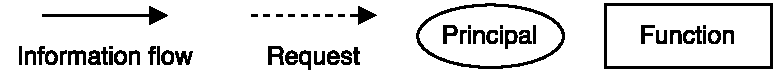
\includegraphics[scale=0.8]{figures/dlm_legend}
  \caption{Information flow graph legend}
  \label{example:legend}
\end{figure}
In the graphs we have two abstractions that are not apparent when looking at the source code.
The main function has been left out, and the \emph{request} flows represent calls to the program, through some means (e.g. a call from another program or through a web-request).
In the code source, the logic in the main function will also not completely represent an actual implementation, as we have abstracted away from how the program will actually be called.

\subsection{Smart meter bill calculation}
Related to the protection of smart meter data, we have created a simple example (see \cref{example:code:calculate_bill} and \cref{example:graph:calculate_bill}) which uses data from both consumer and electrical company in order to calculate a bill.
Here we make use of 4 declared auxiliary functions: \dlmc{get_latest_usage}, \dlmc{get_latest_prices}, \dlmc{send_to_consumer}, and \dlmc{send_to_electrical_company}.
The actual implementation of these is not important, they are only seen to represent ways of either obtaining data from outside the program, or sending data to outside of the program.

\lstinputlisting[float, style=dlmc, numbers=left, caption={Smart meter bill calculation example}, label=example:code:calculate_bill]{dlm_examples/report/calculate_bill.ncif}
\begin{figure}
  \centering
  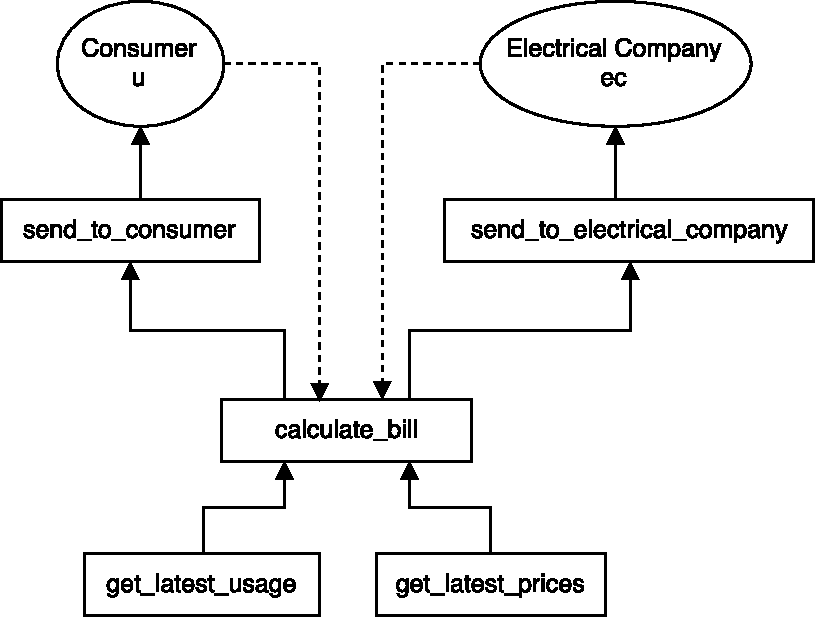
\includegraphics[scale=0.8]{figures/dlm_calculate_bill}
  \caption{Information flow graph for \dlmc{calculate_bill}}
  \label{example:graph:calculate_bill}
\end{figure}

\subsection{Password checker}\label{example:sec:check_password}
A more general example is a password checker (see \cref{example:code:check_password} and \cref{example:graph:check_password}), which takes a username and password combination and checks it against the user database, giving a response to the user whether it was correct or not.
Here we have 3 auxiliary functions: \dlmc{get_login}, \dlmc{get_users}, and \dlmc{send_response} -- they represent the two inputs needed, as well as the response to be given.

\lstinputlisting[float, style=dlmc, numbers=left, caption={Password checker example}, label=example:code:check_password]{dlm_examples/report/check_password.ncif}
\begin{figure}
  \centering
  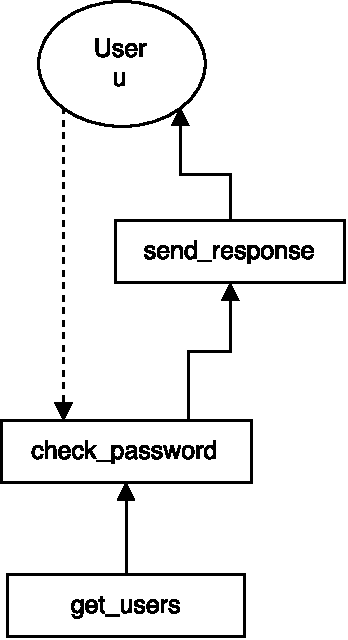
\includegraphics[scale=0.8]{figures/dlm_check_password}
  \caption{Information flow graph for \dlmc{check_password}}
  \label{example:graph:check_password}
\end{figure}
